\section{Experiments}\label{sec:exp}
In this section, we present a comparative analysis of the effectiveness of Sliceformer on multiple tasks. 
The purpose of these experiments is to validate our two hypotheses. 
Firstly, we demonstrate the ability of Sliceformer in modeling Long Range dependencies through the Long Range Arena benchmark, while also showcasing Sliceformer's fast training speed and minimal memory consumption when dealing with long sequences. 
Subsequently, we investigate the numerical stability of Sliceformer by comparing the cosine similarity in the numerical values of the scrambled input representations at different layers in Graphormer. 
Finally, we conduct experiments on Imagenet to verify that even with significantly reduced parameters, Sliceformer still achieves greater capacity than the scaled dot product attention.

\subsection{Comparisons on the Long Range Arena Benchmark}
In order to evaluate the ability of our proposed model to model Long Range dependencies, we conducted experiments on the Long Range Arena benchmark~\cite{tay2021long}. 
Long Range Arena is a benchmark designed to evaluate models under long sequence scenarios, which consists of six tasks, including ListOps~\cite{nangia2018listops}, byte-level text classification~\cite{maas2011learning}, byte-level document retrieval~\cite{radev2013acl}, image classification on CIFAR-10~\cite{krizhevsky2009learning}, Pathfinder~\cite{linsley2018learning}, and Pathfinder-128(a longer and more difficult version of Pathfinder). 
To ensure fairness, we re-implemented our method based on Jax~\cite{bradbury2018jax} and strictly followed the data processing and experimental design of the benchmark.

\begin{table}[htbp]
  \centering
  \caption{The comparison for various models on the Long Range Arena benchmark. FAIL means this method isn't able to converge all the time.}
  % \small{
    \begin{tabular}{l|cccccc|c}
    \toprule
    \multicolumn{1}{c|}{Model} & ListOps & Text  & Retrieval & Image & Path  & Path-X & Avg. Acc\\
    \midrule
    Transformer~\cite{vaswani2017attention} & 36.37 & 64.27 & 57.46 & 42.44 & 71.40 & FAIL  & 54.39 \\
    \midrule
    Local Attention~\cite{tay2021long} & 15.82 & 52.98 & 53.39 & 41.46 & 66.63 & FAIL  & 46.06 \\
    Linear Trans.~\cite{katharopoulos2020transformers} & 16.13 & \textbf{65.90} & 53.09 & 42.34 & 75.30 & FAIL  & 50.55 \\
    Reformer~\cite{kitaev2020reformer}  & 37.27 & 56.10 & 53.40 & 38.07 & 68.50 & FAIL  & 50.67 \\
    Sinkformer~\cite{sander2022sinkformers} & 30.70 & 64.03 &  55.45 & 41.08 & 64.65 & FAIL & 51.18 \\
    Sparse Trans.~\cite{child2019generating} & 17.07 & 63.58 & 59.59& \underline{44.24} & 71.71 & FAIL  & 51.24 \\
    Sinkhorn Trans.~\cite{tay2020sparse} & 33.67 & 61.20 & 53.83 & 41.23 & 67.45 & FAIL  & 51.29 \\
    Linformer~\cite{wang2020linformer} & 35.70 & 53.94 & 52.27 & 38.56 & 76.34 & FAIL  & 51.36 \\
    Performer~\cite{choromanski2021rethinking} & 18.01 & \underline{65.40} & 53.82 & 42.77 & \underline{77.05} & FAIL  & 51.41 \\
    Synthesizer~\cite{tay2021synthesizer} & 36.99 & 61.68 & 54.67 & 41.61 & 69.45 & FAIL  & 52.88 \\
    Longformer~\cite{beltagy2020longformer} & 35.63 & 62.85 & 56.89 & 42.22 & 69.71 & FAIL  & 53.46 \\
    BigBird~\cite{zaheer2020big} & 36.05 & 64.02 & 59.29 & 40.83 & 74.87 & FAIL  & 55.01 \\
    Cosformer~\cite{zhen2022cosformer} & \textbf{37.90} & 63.41 & \underline{61.36} & 43.17 & 70.33 & FAIL  & \underline{55.23} \\
    \midrule
    % Sliceformer & \underline{37.50} &  64.60     &  \textbf{62.23}     &   \textbf{45.96}    &  \textbf{68.52}      &   FAIL  & \textbf{55.76}  \\
    Sliceformer(new) & \underline{37.65} &  64.60     &  \textbf{62.23}     &   \textbf{48.02}    &  \textbf{82.04}      &   FAIL  & \textbf{58.91}  \\
    \bottomrule
    \end{tabular}%
  \label{tab:addlabel}%
  % }
\end{table}%


\begin{table}[htbp]
  \centering
  \caption{The comparison for various models on their computational efficiency. OOM means this method is out of memory in this setting.}
    \begin{tabular}{l|cccc|cccc}
    \toprule
    \multirow{2}{*}{Model}  & \multicolumn{4}{c|}{Train speed(steps per second)}  & \multicolumn{4}{c}{Peak Memory Usage (GB)} \\
     & 1K    & 2K    & 3K    & 4K    &  1K    & 2K    & 3K    & 4K \\
    \midrule
    Transformer~\cite{vaswani2017attention} & 27.49 & 9.45  & 4.73  & OOM & 11.64 & 32.45 & 65.67 &  OOM \\
    \midrule
    Local Attention~\cite{tay2021long} & 31.41 & 25.47 & 18.06 & 13.80 &  6.23  & 9.24  & 12.26 & 15.27 \\
    Linear Trans.~\cite{katharopoulos2020transformers} & 31.35 & 25.79 & 17.07 & 12.32 & 6.50  & 9.84  & 13.18 & 16.52 \\
    Reformer~\cite{kitaev2020reformer} & 31.55 & 22.00 & 13.42 & 8.84  &  6.91  & 12.22 & 19.54 & 28.88 \\
    Sinkformer~\cite{sander2022sinkformers} & 18.72 & 5.82  & 2.86  & OOM  & 14.13 & 41.58 & 82.53 & OOM \\
    Sparse Trans.~\cite{child2019generating} & 27.39 & 9.47  & 4.72  & OOM & 11.64 & 32.45 & 65.71 & OOM \\
    Sinkhorn Trans.~\cite{tay2020sparse} & 29.88 & 22.00 & 15.66 & 11.70 &  6.70  & 10.23 & 13.78 & 17.32 \\
    Linformer~\cite{wang2020linformer} & 28.47 & 28.08 & 19.08 & 14.55 &  5.95  & 8.82  & 11.65 & 14.47 \\
    Performer~\cite{choromanski2021rethinking} & 28.84 & 26.67 & 18.97 & 14.10 & 6.25  & 9.35  & 12.45 & 15.54 \\
    Synthesizer~\cite{tay2021synthesizer} & 19.57 & 6.27  & 3.01  & OOM &  12.77 & 37.53 & 75.23 & OOM  \\
    Longformer~\cite{beltagy2020longformer} & 17.56 & 5.67  & 2.74  &  OOM & 13.00 & 37.07 & 75.46 & OOM\\
    BigBird~\cite{zaheer2020big} & 27.27 & 14.34 & 9.76  & 7.21  & 9.59  & 16.53 & 23.16 & 30.07 \\    
    Cosformer~\cite{zhen2022cosformer} & 32.42 & 26.13 & 17.56 & 12.58 & 6.36 & 9.68 & 13.36 & 16.95 \\
    \midrule
    Sliceformer & 32.79 & 32.26 & 21.79 & 16.25  & 5.61  & 8.12  & 10.64 & 13.14 \\
    \bottomrule
    \end{tabular}%
  \label{tab:addlabel}%
\end{table}%


\textbf{The Necessity of Slice-sorting.}
\xu{Add an analytic experiment to demonstrate the necessity of sorting and the influence of sorting times. 
Compare $\text{Sort}_{\text{col}}(\bm{V})$, $\bm{V}$, and $\text{Sort}(\bm{V})$ twice.}


\subsection{Comparisons on ImageNet}
dataset: CIFAR10 64x64 128x128 CIFAR100 64x64 128x128
methods: transformer sliceformer

\subsection{Numerical Stability Analysis}
As is well-known, the $\text{Softmax}()$ in conventional scaled dot product attention is a row-wise function and theoretically equivariant to row permutations. 
However, in our experiments, as shown in the figure~\ref{fig:cos}, we found that the $\text{Softmax}()$ has poor permutation equivariance, which may be due to the implementation details, and introduces significant numerical errors. 
Moreover, the numerical errors accumulate at each layer, which severely limits the performance of deep Transformer networks. 
By removing the $\text{Softmax}()$, our proposed method greatly reduces the numerical errors and exhibits perfect numerical stability.

\begin{figure}
  \centering
    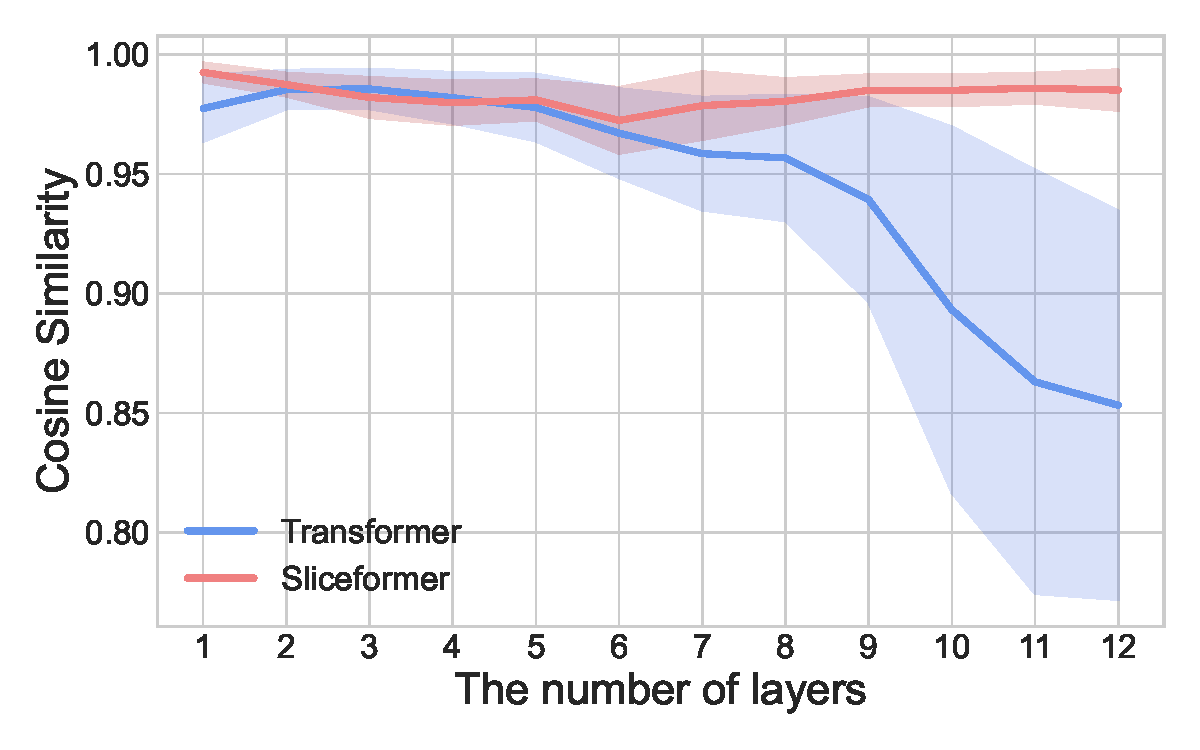
\includegraphics[width=0.8\textwidth]{figures/cos_sim.pdf}
    \caption{Comparison of the numerical stability of different layers in the Graphormer model with our method and the Transformer. The cumulative error in Transformer increases with the number of layers, while our method avoids introducing unexpected numerical errors by removing the softmax function.}
    \label{fig:cos}
\end{figure}

\subsection{Comparisons on Long Sequences}

\subsection{Ablation Study on the Sorting Times}


% Table generated by Excel2LaTeX from sheet 'SortTimes'
\begin{table}[htbp]
  \centering
  \caption{Performance comparison of sorting times. Sliceformer-softmax: learnable weights with Softmax(). Sliceformer-fixed: average.}
    \begin{tabular}{l|cccc}
    \toprule
    Method & 2     & 3     & 4     & 8 \\
    \midrule
    Sliceformer-softmax & 80.15 & 80.61 & 79.65 & 77.07 \\
    Sliceformer-fixed & 80.29 & 78.85 & 78.55 & 77.64 \\
    \bottomrule
    \end{tabular}%
  \label{tab:addlabel}%
\end{table}%

\subsection{Ablation Study on the Sorting Order}

Table~\ref{tab:order} compares the effect of different sorting orders on model performance in the LRA benchmark. 
We tried four sorting orders: Ascending, Descending, Half Half(half columns in ascending order and half in descending order), and Shuffle(column-wise). 
Evidently, except for the last one, the results of the other three sorting orders are very close, indicating that Sliceformer is robust to the specific order of each column. 
However, for the randomly shuffle, Sliceformer clearly loses its learning ability and degenerates into a randomly selecting model.

% Table generated by Excel2LaTeX from sheet 'Order'
\begin{table}[htbp]
  \centering
  \caption{Performance comparison of sorting order.}
    \begin{tabular}{l|cccccc|c}
    \toprule
    \multicolumn{1}{c|}{Sorting Order} & ListOps & Text  & Retrieval & Image & Path  & Path-X & Avg \\
    \midrule
    Ascending & 37.65 & 64.60 & 62.23 & 48.02 & 82.04 & FAIL  & 58.91 \\
    Descending & 37.50 & 64.36 & 61.95 & 45.46 & 81.70 & FAIL  & 58.19 \\
    Half  Half  & 37.45 & 64.25 & 61.95 & 45.80 & 81.38 & FAIL  & 58.17 \\
    Shuffle & 17.85 & 50.49 & 50.87 & 10.00 & 49.74 & FAIL  & 35.79 \\
    \bottomrule
    \end{tabular}%
  \label{tab:order}%
\end{table}%

% Table generated by Excel2LaTeX from sheet 'pooling'
\begin{table}[htbp]
  \centering
  \caption{Add caption}
    \begin{tabular}{l|cccccc|c}
    \toprule
    \multicolumn{1}{c|}{Model} & ListOps & Text  & Retrieval & Image & Path  & Path-X & Avg \\
    \midrule
    Sliceformer & 37.65 & 64.60  & 62.23 & 48.02 & 82.04 & FAIL  & 58.91 \\
    Min pooling & 36.95 & 62.82 & 60.33 & 40.02 & 74.77 & FAIL  & 54.98 \\
    Max pooling & 36.80 & 62.88 & 60.90 & 40.54 & 74.62 & FAIL  & 55.15 \\
    Max abs with sign & 38.15 & 62.61 & 60.78 & 39.27 & 74.93 & FAIL  & 55.15 \\
    Max abs & 37.15 & 63.08 & 59.51 & 36.67 & 73.37 & FAIL  & 53.96 \\
    Max exchange & 37.00 & 62.90 & 59.00 & 40.48 & 75.42 & FAIL  & 54.96 \\
    \bottomrule
    \end{tabular}%
  \label{tab:addlabel}%
\end{table}%



